\section{Search for eV-scale Sterile Neutrinos}
\label{sec:sterile-measurement}

This analysis assumes the extended 3+1 neutrino PMNS framework, with the parameters to be constrained being the oscillation parameters $\theta_{24}$ and $\theta_{34}$. The three-flavor atmospheric oscillation parameters and the CP-violating phase $\delta_{24}$ are treated as nuisance parameters. The mass splitting of the additional mass eigenstate is fixed at $\Delta m^2_{41}=1\;\mathrm{eV^2}$. Because the oscillations at Earth-scale baselines happen on much smaller energy scales than can be resolved by DeepCore, the analysis effectively becomes indifferent to the magnitude of $\Delta m^2_{41}$ and constrains the values of $\theta_{24}$ and $\theta_{34}$ based on the \emph{averaged} oscillation effect. As a consequence, constraints calculated based on the assumption that $\Delta m^2_{41}=1\;\mathrm{eV^2}$ are still valid even if the true mass splitting is much larger. This holds true up to mass splitting values of about $m^2_{41}\gtrapprox100\;\mathrm{eV^2}$, where the heavy mass eigenstate becomes so much slower than the light eigenstates that it would no longer interfere with them and decohere\sidecite{atmo_decoherence}.

\subsection{The 3+1 model}
This analysis probes the "3+1" oscillation model, in which a fourth "sterile" (i.e. non-interacting) neutrino flavor eigenstate $\nu_s$ and mass eigenstate $\nu_4$ with mass splitting $\Delta m^2_{41}$ is added to the standard three-flavor model. This state The PNMS mixing matrix is extended by a fourth row and column, which is parametrized with additional mixing angles $\theta_{14}$, $\theta_{24}$, $\theta_{34}$ and CP violating phases $\delta_{14}$ and $\delta_{24}$ as
\begin{align*}
    U_{3+1} =&\begin{pmatrix}
    U_{e1}    & U_{e2}    & U_{e3}   &U_{e4}    \\
    U_{\mu1}  & U_{\mu2}  & U_{\mu3} &U_{\mu4}  \\
    U_{\tau1} & U_{\tau2} & U_{\tau3}&U_{\tau4} \\
    U_{s1} & U_{s2} & U_{s3}&U_{s4} \\
    \end{pmatrix}\\
    =&
    R_{34}(\theta_{34})
    \tilde{R}_{24}(\theta_{24}, \delta_{24})
    \tilde{R}_{14}(\theta_{14}, \delta_{14})
    R_{23}(\theta_{23})
    \tilde{R}_{13}(\theta_{13}, \delta_{13})
    R_{12}({\theta_{12})}\;,
\end{align*}
where $R_{kl}$ are rotation matrices. The goal of this analysis is to constrain the matrix elements $U_{\mu4}$ and $U_{\tau4}$ with magnitude $|U_{\mu4}|^2=\sin^2(\theta_{24})$ and  $|U_{\tau4}|^2=\sin^2(\theta_{34})\cos^2\theta_{24}$, respectively, via the measurement of $\nu_\mu$ disappearance.

\subsection{Atmospheric oscillations in the presence of an eV-scale sterile neutrino}
In the presence of an eV-scale sterile neutrino, the standard three-flavor oscillation pattern as a function of neutrino energy and zenith angle is distorted and overlaid with a much faster secondary oscillation pattern. Figure~\ref{fig:numu_survival_0.5eV2_full_range} shows the muon neutrino survival probability in the presence of a fourth mass eigenstate with $\Delta m^2_{41}=0.5\;\mathrm{eV^2}$ and $\theta_{24}=15^\circ$ as a function of the energy and cosine of the zenith angle, where $\cos(\theta_z)=-1$ indicates that the neutrino is coming directly from below and $\cos(\theta_z)=1$ directly from above. For up-going neutrinos, the oscillation pattern induced by $\Delta m^2_{41}$ is only resolved at energies of $>\mathcal{O}(1\;\mathrm{TeV})$. Below 100~GeV, the oscillation length reaches values of as low as $\mathcal{O}(\mathrm{km})$, which makes them unresolvable below the horizon where baselines are of $\mathcal{O}(10000\;\mathrm{km})$.

\subsubsection{Neutrino production height effects}
Above the horizon, the distance from the upper layers of the atmosphere where the neutrinos are produced to the detector is small enough to create a distinct oscillation pattern for a fixed production height as can be seen in the left panel of figure~\ref{fig:numu_survival_0.5eV2_full_range}. Because neutrino production heights vary over a range of tens of kilometers, it is necessary to average the oscillation probability over production heights to get a more realistic expectation. This is done analytically in \texttt{nuSQuIDS} by calculating the averaged vacuum oscillation probability over a uniform distribution. The right panel of figure~\ref{fig:numu_survival_0.5eV2_full_range} shows the oscillation probability with production heights averaged between 10~km and 30~km. The oscillation pattern above the horizon is no longer clearly resolvable, but an average disappearance effect for neutrino energies below 20~GeV remains. The uniform distribution that is assumed to calculate the averaged oscillation probabilities is of course not entirely realistic. For this reason, only events arriving at most slightly above the horizon ($\cos(\theta_z)<0.1$) are included in this analysis
\begin{figure}
    \centering
    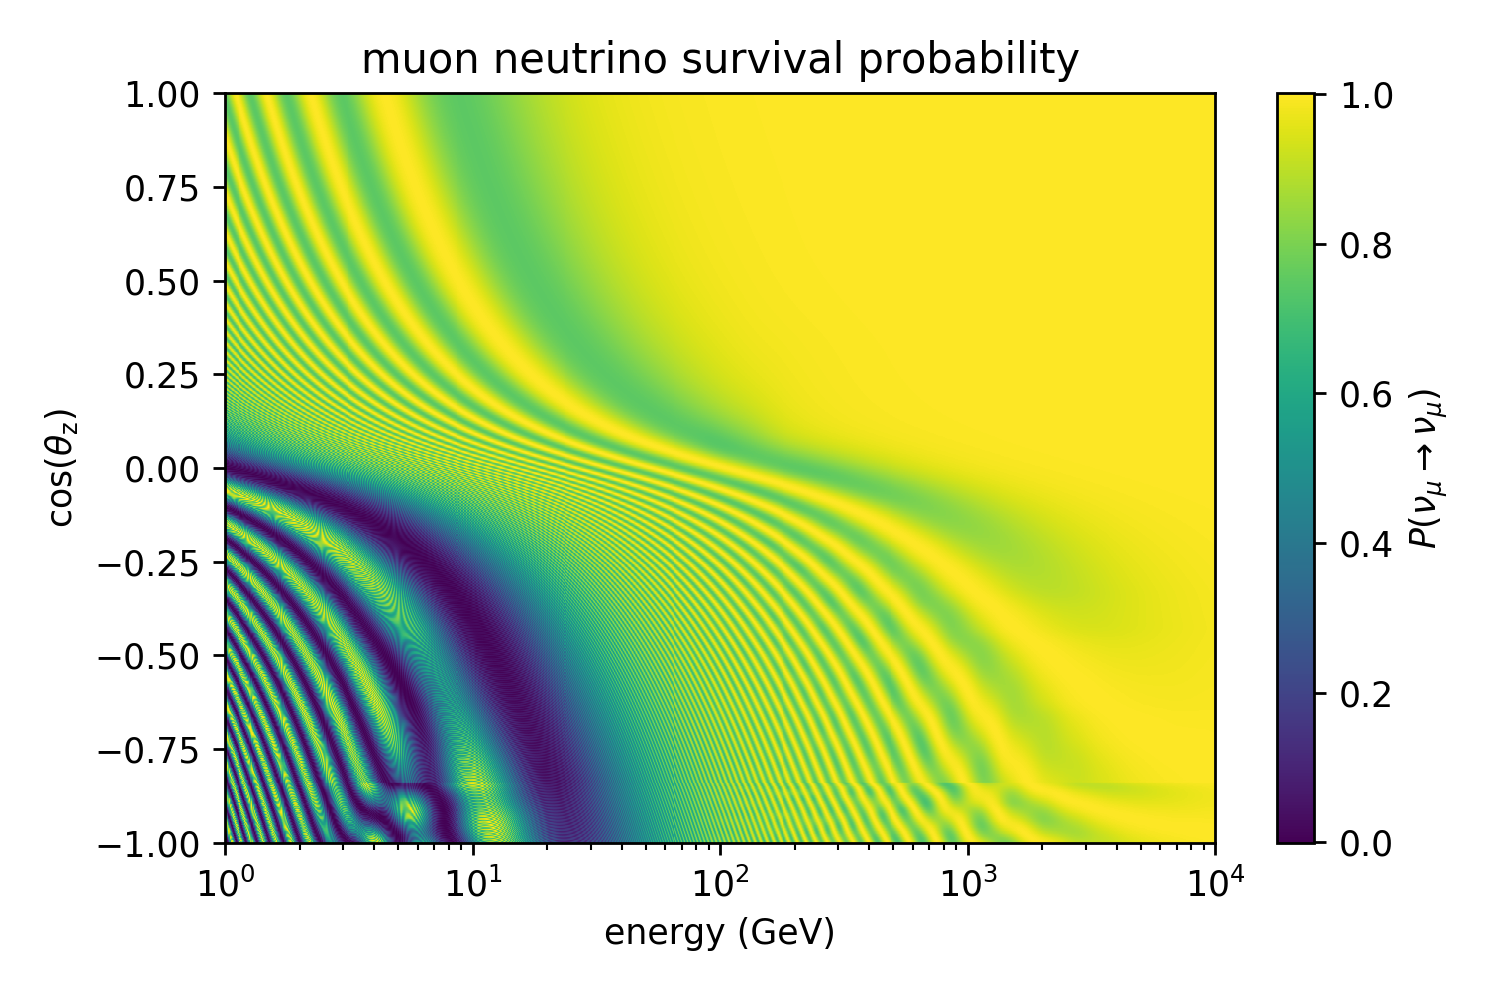
\includegraphics[width=0.49\textwidth]{figures/measurement/sterile_analysis/physics/dm41_0.5eV2_th24_15deg_no_filter.png}
    \hfill
    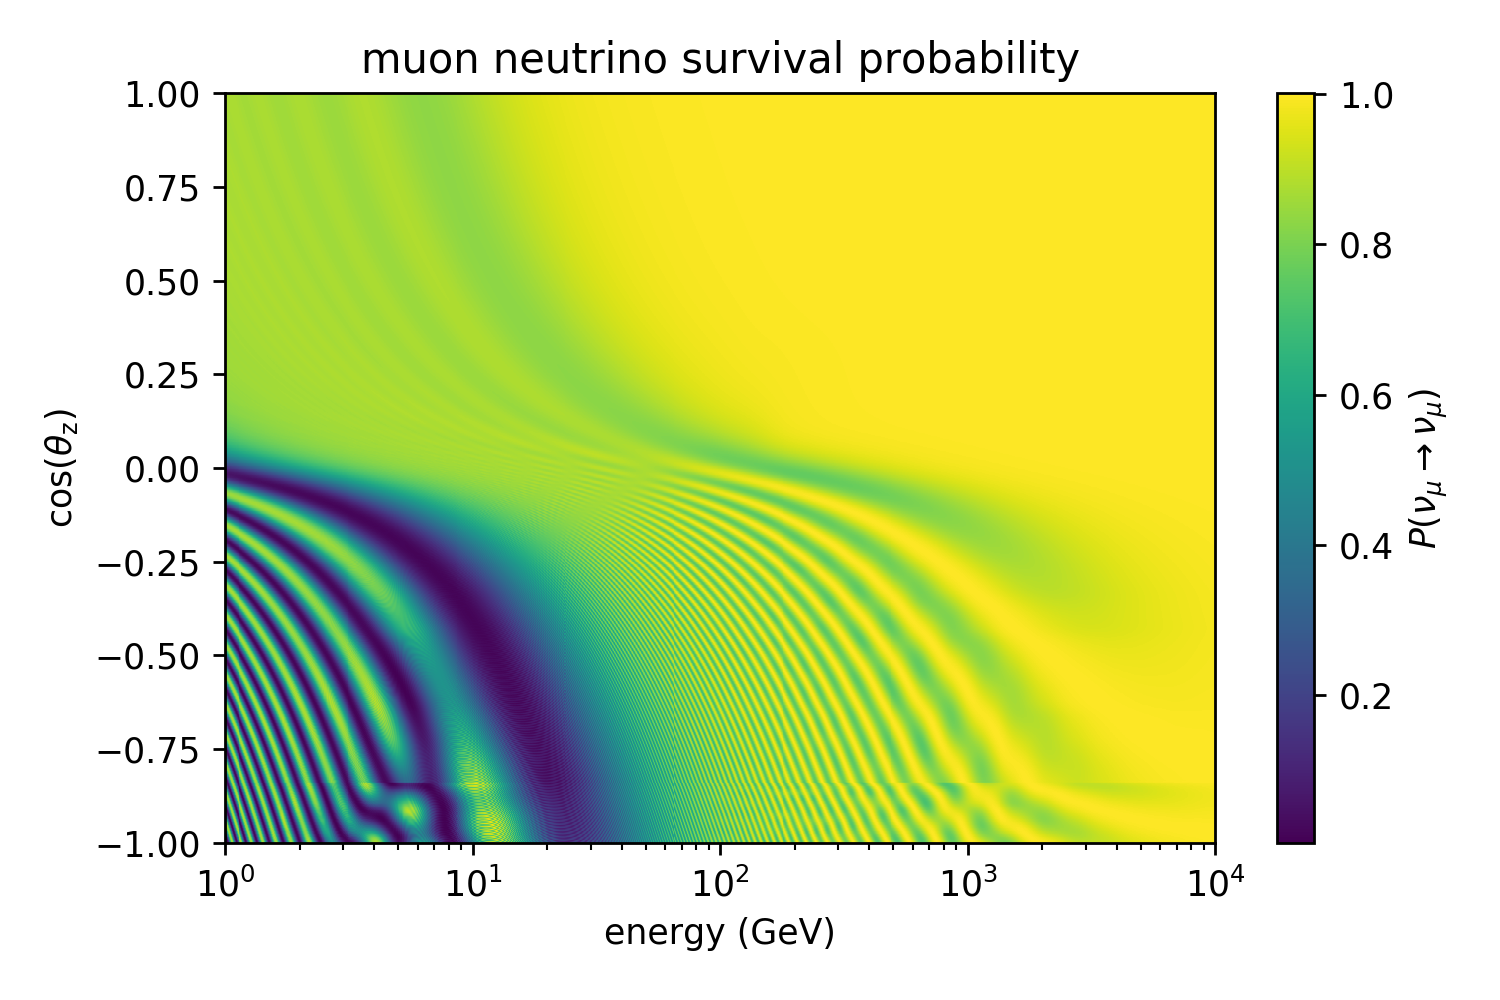
\includegraphics[width=0.49\textwidth]{figures/measurement/sterile_analysis/physics/dm41_0.5eV2_th24_15deg_avg_height_10-30km.png}
    \caption{Muon neutrino survival probability in the presence of a fourth mass eigenstate with $\Delta m^2_{41}=0.5\;\mathrm{eV^2}$ and $\theta_{24}=15^\circ$ with a fixed production height of 20~km (left) and with production heights averaged between 10~km and 30~km (right).}
    \label{fig:numu_survival_0.5eV2_full_range}
\end{figure}

\subsubsection{Oscillation signal for large mass splittings}
In the mass-splitting range where $\Delta m_{41}\approx\mathcal{O}(1\,\mathrm{eV^2})$ and in the energy range of the event sample ($<150\;\mathrm{GeV}$), the presence of a sterile neutrino produces rapid oscillations overlaid on the standard three-flavor oscillation pattern as well as distortions to that pattern itself as shown in figure~\ref{fig:numu_survival_1eV2_analysis_binning_range} for a mixing angle of $\theta_{24}=15^\circ$. The oscillation frequency in energy is too large to be resolved by DeepCore, but the average effect still allows constraining the magnitudes of the $U_{\mu4}$ and $U_{\tau4}$. The precise value of $\Delta m^2_{41}$ has very little influence on the average amplitude of the oscillations and therefore cannot be recovered in this mass splitting regime. The oscillation averages stay approximately constant up to mass splitting values of well above $100\;\mathrm{eV^2}$ where decoherence effects begin to play a role\cite{atmo_decoherence}.
\begin{figure}
    \centering
    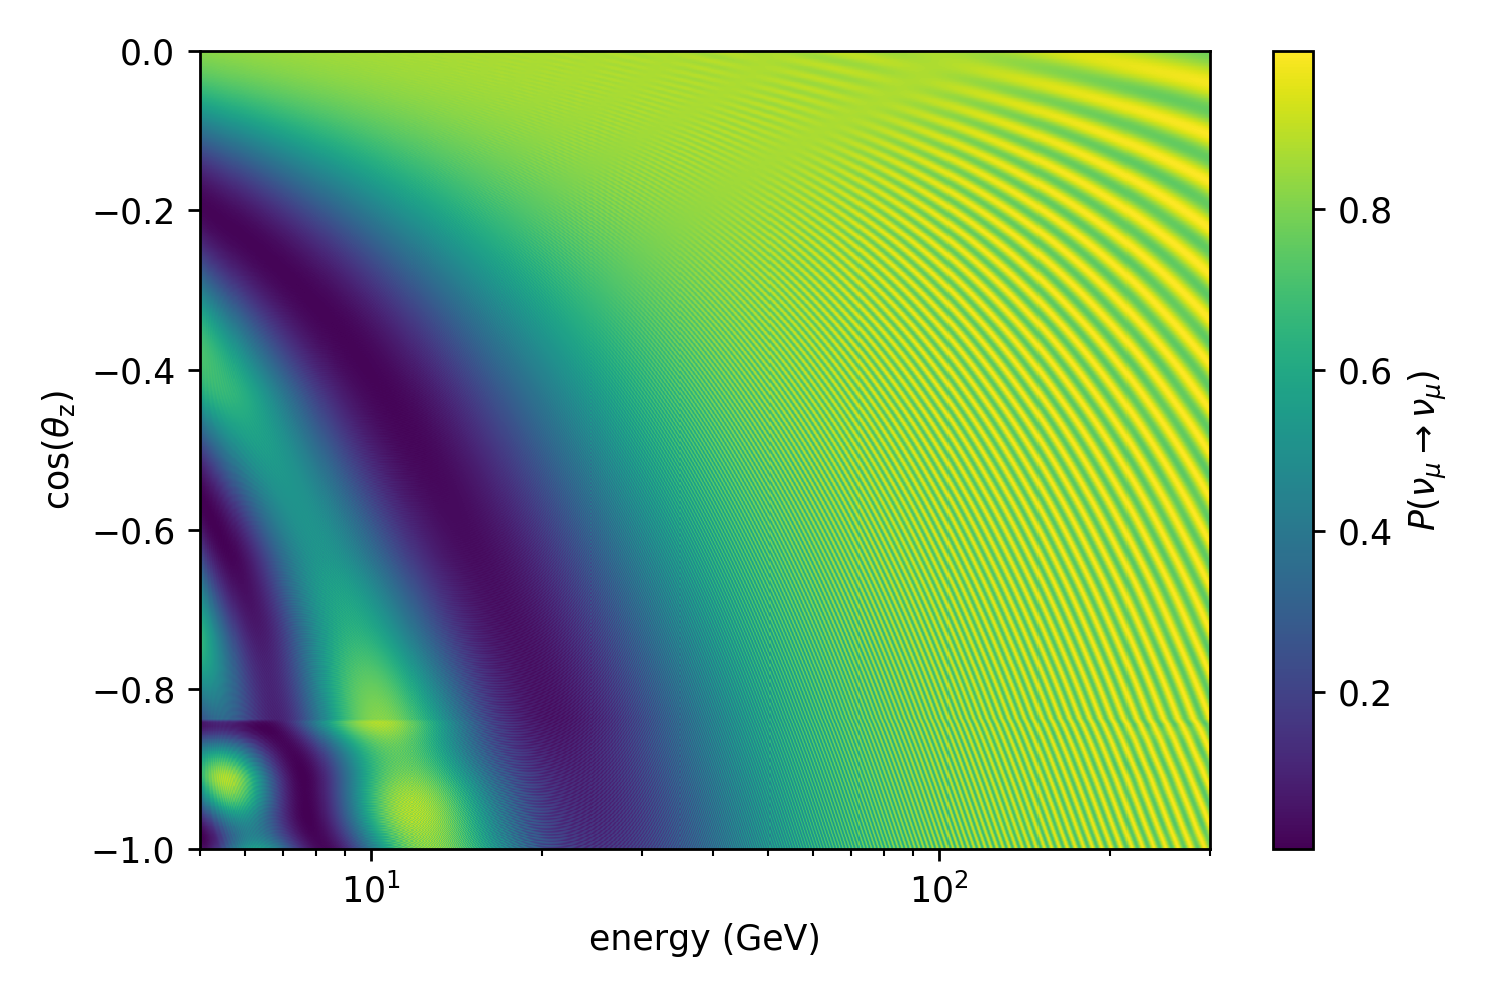
\includegraphics[width=0.8\textwidth]{figures/measurement/sterile_analysis/physics/dm41_1.0eV2_th24_15deg_avg_height_10-30km_ana_binning_range.png}
    \caption{$\nu_{\mu}$ survival probability at $\Delta m^2_{41}=1\;\mathrm{eV^2}$ and $\theta_{24}=15^\circ$}
    \label{fig:numu_survival_1eV2_analysis_binning_range}
\end{figure}

\subsubsection{Oscillation signal for small mass splittings}
For mass-splitting values of $\Delta m^2_{41}$ well below $1\;\mathrm{eV^2}$, the oscillation pattern is no longer completely averaged out. Figure~\ref{fig:numu_survival_0.1eV2_analysis_binning_range} shows the muon-neutrino survival probability in the presence of a sterile neutrino state with mass splitting $\Delta m^2_{41}=0.1\;\mathrm{eV^2}$ and mixing angle $\theta_{24}=15^\circ$. The highest oscillation minimum in energy and cosine of the zenith angle (upper right corner of the figure) is large enough to be resolvable with DeepCore. This makes it possible in principle to produce constraints of the mixing matrix elements as a function of the mass-splitting $\Delta m^2_{41}$, although this is beyond the scope of the analysis presented in this thesis.
\begin{figure}
    \centering
    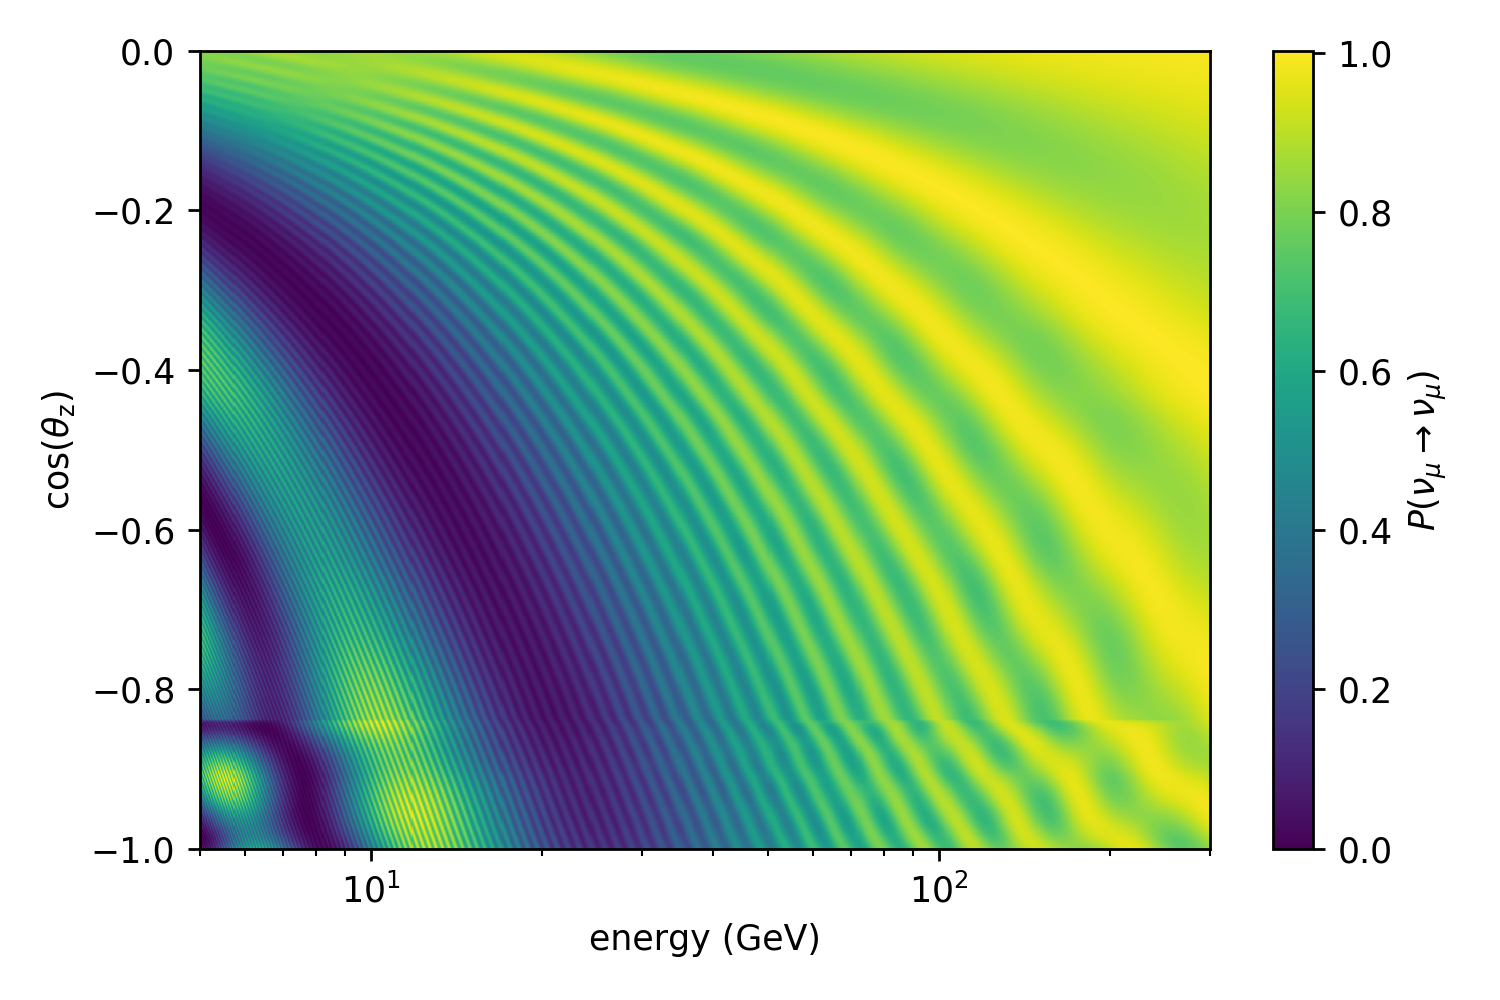
\includegraphics[width=0.8\textwidth]{figures/measurement/sterile_analysis/physics/dm41_0.1eV2_th24_15deg_avg_height_10-30km_ana_binning_range.png}
    \caption{$\nu_{\mu}$ survival probability at $\Delta m^2_{41}=0.1\;\mathrm{eV^2}$ and $\theta_{24}=15^\circ$}
    \label{fig:numu_survival_0.1eV2_analysis_binning_range}
\end{figure}

\subsection{Nuisance oscillation parameters}
Besides the physics parameters $\theta_{24}$ and $\theta_{34}$ to be constrained by the analysis (at a fixed sterile mass splitting $\Delta m^2_{14}$), there are 4 additional mixing angles and 3 CP-violating phases in the 3+1 PNMS matrix as well as the mass splittings $\Delta m^2_{12}$ and $\Delta m^2_{13}$ that influence the oscillation probability. The solar and reactor angles $\theta_{12}$ and $\theta_{13}$ as well as the solar mass splitting $\Delta m^2_{12}$ are constrained by other experiments beyond the sensitivity of this analysis and are fixed at their current global best fit point\sidecite{nufit40}. The effect of the standard three-flavor CP violating phase $\delta_{\mathrm{CP}}=\delta_{13}$ is negligible and it is fixed to zero. The mixing angle $\theta_{14}$ and the phase $\delta_{14}$ are also fixed to zero, since recent reactor data constrains $|U_{e4}|^2 = \sin^2(\theta_{14})$ to $\mathcal{O}(10^{-3})$, which is well below the sensitivity of this analysis\sidecite{global_unitarity_Hu}. The only nuisance parameters that remain free are the standard 3-flavor atmospheric oscillation parameters $\theta_{23}$ and $\Delta m^2_{13}$ as well as the sterile CP-violating phase $\delta_{24}$. The effect of $\delta_{24}$ is to shift the oscillation pattern of muon neutrinos as shown in figure~\ref{fig:sterile-cp-phase-effect}. The effect for \emph{anti}neutrinos runs in the opposite direction. Because neutrinos and antineutrinos are nearly indistinguishable in DeepCore, the combined effect of $\delta_{24}$ is a smearing of the oscillation minimum. Additionally, the sign of $\cos(\delta_{24})$ is approximately degenerate with the neutrino mass hierarchy effect. It's therefore expected that the analysis will produce very similar results for NO and IO when $\delta_{24}$ is free. Table~\ref{tab:oscillation-parameters} gives an overview over all oscillation parameters in the 3+1 model and their treatment in this analysis.
\begin{figure}
    \centering
    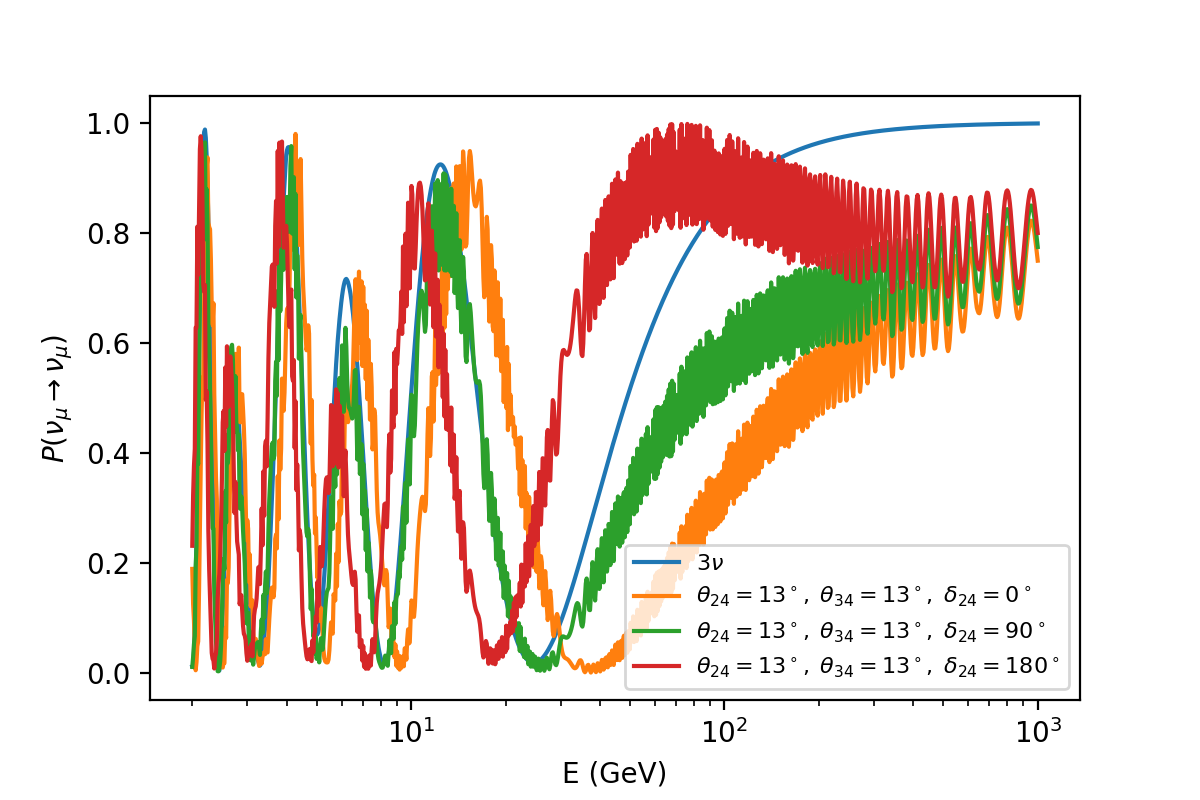
\includegraphics[width=0.8\textwidth]{figures/measurement/sterile_analysis/physics/Muon_neutrino_survival_probability_with_steriles_1D.png}
    \caption{Muon neutrino survival probability for a directly up-going neutrino as a function of energy in the presence of sterile neutrinos at different values of the sterile CP violating phase.}
    \label{fig:sterile-cp-phase-effect}
\end{figure}

\begin{table}
    \centering
    \begin{tabular}{@{}cccp{0.35 \linewidth}@{}}\toprule
        \textbf{parameter} & \textbf{nominal value} & \textbf{fixed?} & \textbf{comment} \\
        \midrule
        $\theta_{14}$ & $0^\circ$ & fixed &  Constr. by reactor data \\
        $\theta_{24}$ & -- & free & Physics parameter\\
        $\theta_{34}$ & -- & free & Physics parameter\\
        $\theta_{12}$ & $33.82^\circ$ & fixed & Constrained by reactor and solar data \\
        $\theta_{13}$ & $8.61^\circ$ & fixed & Constrained by reactor and accelerator data \\
        $\theta_{23}$ & $49.6^\circ$ & free & Atm. mixing angle \\
        $\delta_{13}$ & $0^\circ$ & fixed &  Negligible effect \\
        $\delta_{14}$ & $0^\circ$ & fixed &  No effect when $\theta_{14} = 0^\circ$ \\
        $\delta_{24}$ & -- & free & Smears osc. minimum \\
        $\Delta m^2_{21}$ & $7.39\times10^{-5}\;\mathrm{eV^2}$ & fixed & Constrained by reactor and solar data \\
        $\Delta m^2_{31}$ & $2.525\times10^{-3}\;\mathrm{eV^2}$ & free & Atm. mass splitting \\
        $\Delta m^2_{41}$ & $1\;\mathrm{eV^2}$ & fixed & Averaged out above $1\;\mathrm{eV^2}$ \\
        \bottomrule
    \end{tabular}
    \caption{Oscillation parameters of the 3+1 model and their treatment in this analysis.}
    \label{tab:oscillation-parameters}
\end{table}

\subsection{Oscillation Probability Calculation with nuSQuIDS}
\label{sec:nusquids}

This analysis uses as customized version of \href{https://github.com/ts4051/nuSQuIDS}{nuSQuIDS} that is optimized for the integration into \href{https://github.com/icecube/pisa}{PISA}.\todo{Remove jargon, add proper citation} The basic principle behind nuSQuIDS is to calculate state transition probabilities in the Interaction (Dirac) Picture of quantum mechanics, where the full, time dependent Hamiltonian is split into the time-independent vacuum oscillation part $H_0$ and the time-dependent interaction part $ H_1(t)$:
$$ H(t) = H_0 = H_1(t)$$
In this picture, operators evolve with $ H_0$ as
$$
\bar{O}_I(t)=e^{iH_0t}O_Se^{-iH_0t}\,,
$$
while state densities evolve with the interaction Hamiltonian $ H_1(t)$
$$
\partial_t\bar{\rho}_I(t)=-i[\bar{H}_{1, I}(t), \bar{\rho}_I(t)]\,.
$$

This state evolution is solved via numerical integration in nuSQuIDS, which is computationally expensive. However, because fast oscillations inside $ H_0$ only play a sub-leading role, this difficult calculation does not have to be performed at every point in the analysis space. It is sufficient to calculate state densities at a selected set of points, referred to as \emph{nodes}, and to then interpolate the densities between them. The fast oscillations between the nuSQuIDS nodes are recovered when the probabilities for each flavor, $i$, are projected out with the trace operation on the state density with the (time-evolved) projection operator for that state:
$$
p_i(t)=\mathrm{Tr}(\underbrace{\bar{\Pi}^{(i)}(t)}_{\mathrm{proj.\,op.}}\bar{\rho}_I(t))
$$

\subsubsection{Node placement}
The nodes where the difficult state integration is calculated need not be placed dense enough in the analysis space to resolve the fast oscillations due to sterile neutrinos, but they do need to resolve matter effects. The state densities change most rapidly (as function of energy) for neutrinos that traverse a lot of matter at low energies. Additionally, there is a sharp break at $\cos(\theta_{\mathrm{zenith}})=-0.84$ where neutrinos begin to pass through the core. For this reason, the nuSQuIDs nodes are concentrated in three places:
\begin{itemize}
    \item the energy region between 2 GeV and 10 GeV
    \item within a small interval around $\cos(\theta_{\mathrm{zenith}})=-0.84$
    \item the region below $\cos(\theta_{\mathrm{zenith}})=-0.84$
\end{itemize}
Figure~\ref{fig:nusquids-nodes} shows the optimized placement of nuSQuIDS nodes as black dots.

\begin{figure}
    \centering
    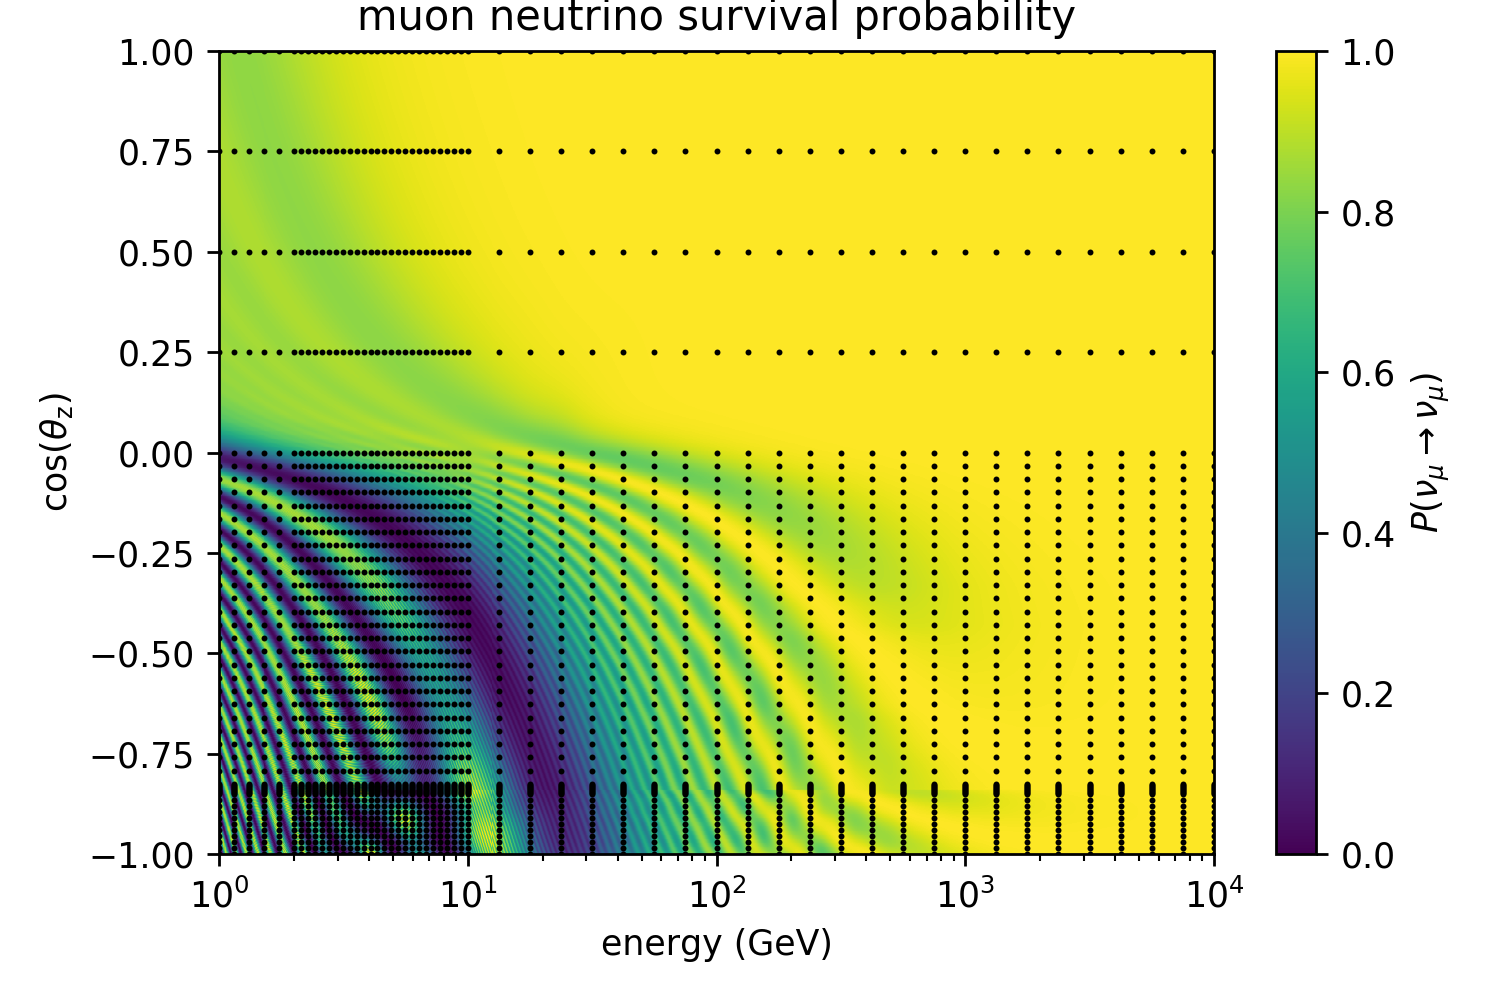
\includegraphics[width=0.7\textwidth]{figures/measurement/sterile_analysis/nusquids/0.1eV_sterile_only_height_avg_optim_nodes.png}
    \caption{Optimized placement of nuSQuIDS nodes (black dots) with extra dense node spacing in the three critical regions. The injected value for $\Delta m^2_{41}$ is $0.1\;\mathrm{eV^2}$.}
    \label{fig:nusquids-nodes}
\end{figure}

\subsubsection{Production height averaging}
At eV-scale mass splittings, oscillations are fast enough that significant oscillations occur even at 10-km-scale distances. If the production height is assumed to be fixed at an exact position, a strong oscillation pattern appears above the horizon that could falsely produce a very high sensitivity in the analysis, driven entirely by events above the horizon. In reality, production heights can vary within the atmosphere, which smears out the oscillations. For this analysis, an analytical averaging method was implemented in nuSQuIDS that assumes a uniform distribution of propagation distances between two points. The start and end point depends on the zenith angle and corresponds to the intersection of the neutrino path with a height of 10 km and 30 km, respectively.

\subsubsection{Low-pass filtering}
\label{sec:low-pass-filtering}
The fast oscillations in the presence of sterile neutrinos are filtered with a low-pass filter both during the state evolution and the calculation of probabilities. This step dramatically increases the speed at which oscillation probabilities can be evaluated.

Vacuum oscillations enter the differential equation governing the state evolution via the time evolution of the interaction Hamiltonian $\bar{H}_{1, I}(t)$. At low energies they cause tiny, but extremely fast oscillations of the time derivative that the numerical integrator has to keep track of by drastically reducing the step size, slowing down the calculation. To mitigate this problem and increase performance, a low-pass filter is applied when calculating the RHS of the differential equation.

\begin{figure}
    \centering
    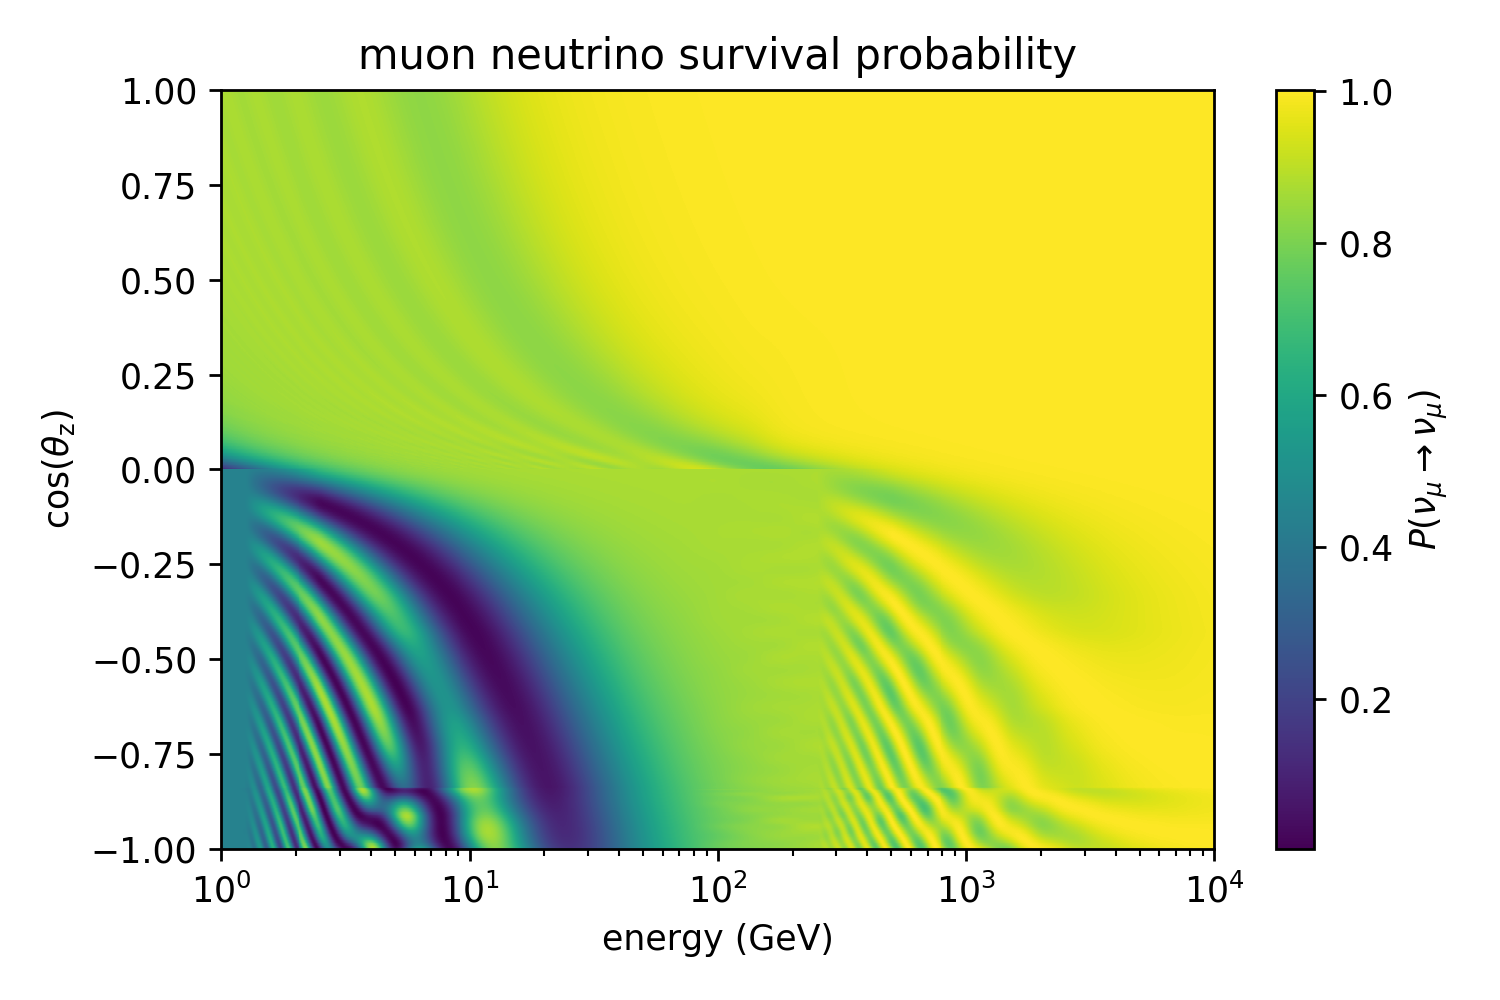
\includegraphics[width=0.7\textwidth]{figures/measurement/sterile_analysis/nusquids/Dm41_0.5eV2_th24_15deg_avg_height_10-30km_lp_belowhor.png}
    \caption{Muon neutrino survival probability in the presence of a sterile neutrino after application of both height averaging and low-pass filtering.}
    \label{fig:nusquids-low-pass-filtering}
\end{figure}

In the presence of sterile oscillations, transition probabilities usually have to be calculated for every single simulated event to average them out in the analysis binning. Because the MC set has millions of events, doing this would be very expensive even when using nuSQuIDs' state interpolation feature. In this analysis, a low-pass filter as a function of energy is applied when the transition probabilities are projected out from the state densities to average out very fast oscillations. With this filtering, it is possible to calculate oscillation probabilities on a fine binning with ~20k bins. One caveat is that this filtering is not appropriate to apply above the horizon because propagation distances there are short enough that oscillation probabilities don't average out completely. It is therefore only applied below the horizon as shown in figure~\ref{fig:nusquids-low-pass-filtering}.


\subsection{Sterile signal in analysis binning}
The change in bin counts with respect to the nominal expectation for different combinations of sterile mixing angles at $\Delta m^2_{41}=1\;\mathrm{eV^2}$ is shown in figure~\ref{fig:oscillation-effects-ana-binning}. While a pull in only $\theta_{34}$ by $20^\circ$ has only a very small effect (see middle panels of figure~\ref{fig:oscillation-effects-ana-binning}), the combination of both angles can greatly amplify the signal. The CP-violating phase $\delta_{24}$ only plays a role when both angles $\theta_{24}$ and $\theta_{34}$ are non-zero. The sensitivity of this analysis to $\theta_{34}$ is entirely due to matter effects experienced by neutrinos passing through the dense core of the Earth.

\begin{figure}
    \centering
    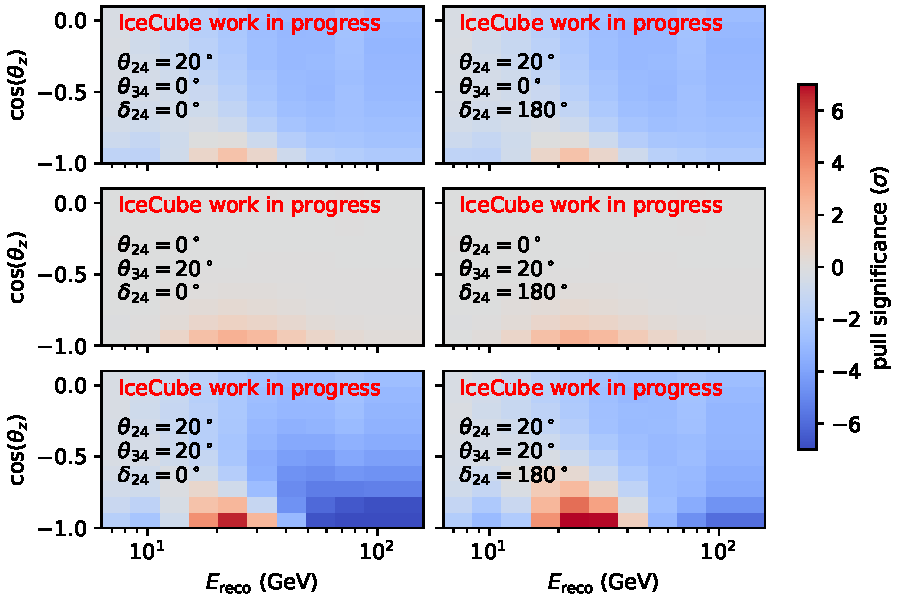
\includegraphics[width=0.95\textwidth]{figures/measurement/sterile_analysis/oscillation_signal/pull_theta_combinations_20deg_dcp24.pdf}
    \caption{Signal in the analysis binning produced by different combinations of $\theta_{24}$, $\theta_{34}$, and $\delta_{24}$ as a fraction of the Poisson error in each bin. The mass splitting of the sterile state is $\Delta m^2_{41}=1\;\mathrm{eV^2}$.}
    \label{fig:oscillation-effects-ana-binning}
\end{figure}

\subsection{Selection of Free Parameters}
\label{sec:sterile-analysis-parameter-selection}
To reduce the computational cost of optimizing the likelihood in a high-dimensional space, the impact of each nuisance parameter in consideration is assessed and its value fixed if it is found to be negligible. Since the standard three-flavor oscillation model is a nested hypothesis within the 3+1 model, the parameter selection described in section~\ref{sec:std-osc-free-parameters} is taken as a starting point for the parameter selection of this analysis.
Starting from that selection, a test is run to determine if a paraemter is entirely dominated by its prior. For this test, 200 trials are run where all nuisance parameters are sampled randomly according to their prior. Then,  Asimov pseudo-data is produced at that point, and this pseudo-data is fit back with the default fit settings. The resulting pairs of true injected parameter values and fitted values for every free parameter are shown in a scatter plot in figure~\ref{fig:parameter-ensemble-result}. If a parameter is entirely dominated by its prior, it will fit back to its nominal value regardless of the injected value. For parameters where this is the case, their value is fixed to their nominal value during a fit. Parameters to which this applies are framed in red in figure~\ref{fig:parameter-ensemble-result}. The framed parameters are (from top to bottom, and from left to right in the bottom row): \texttt{barr\_w\_K}, \texttt{barr\_w\_antiK}, \texttt{barr\_g\_Pi}, \texttt{pion\_ratio}, \texttt{barr\_h\_Pi}. The test shown in the figure was run before the priors on \texttt{barr\_i\_Pi}, \texttt{barr\_z\_K}, and \texttt{barr\_z\_antiK} have been inflated as described in section~\ref{section:flux_systs}. After that change,  \texttt{barr\_i\_Pi} was also added to the set of free parameters of the analysis. The full list of free parameters with their respective ranges and priors is shown in table~\ref{tab:all-parameters}.

\begin{figure*}
    \centering
    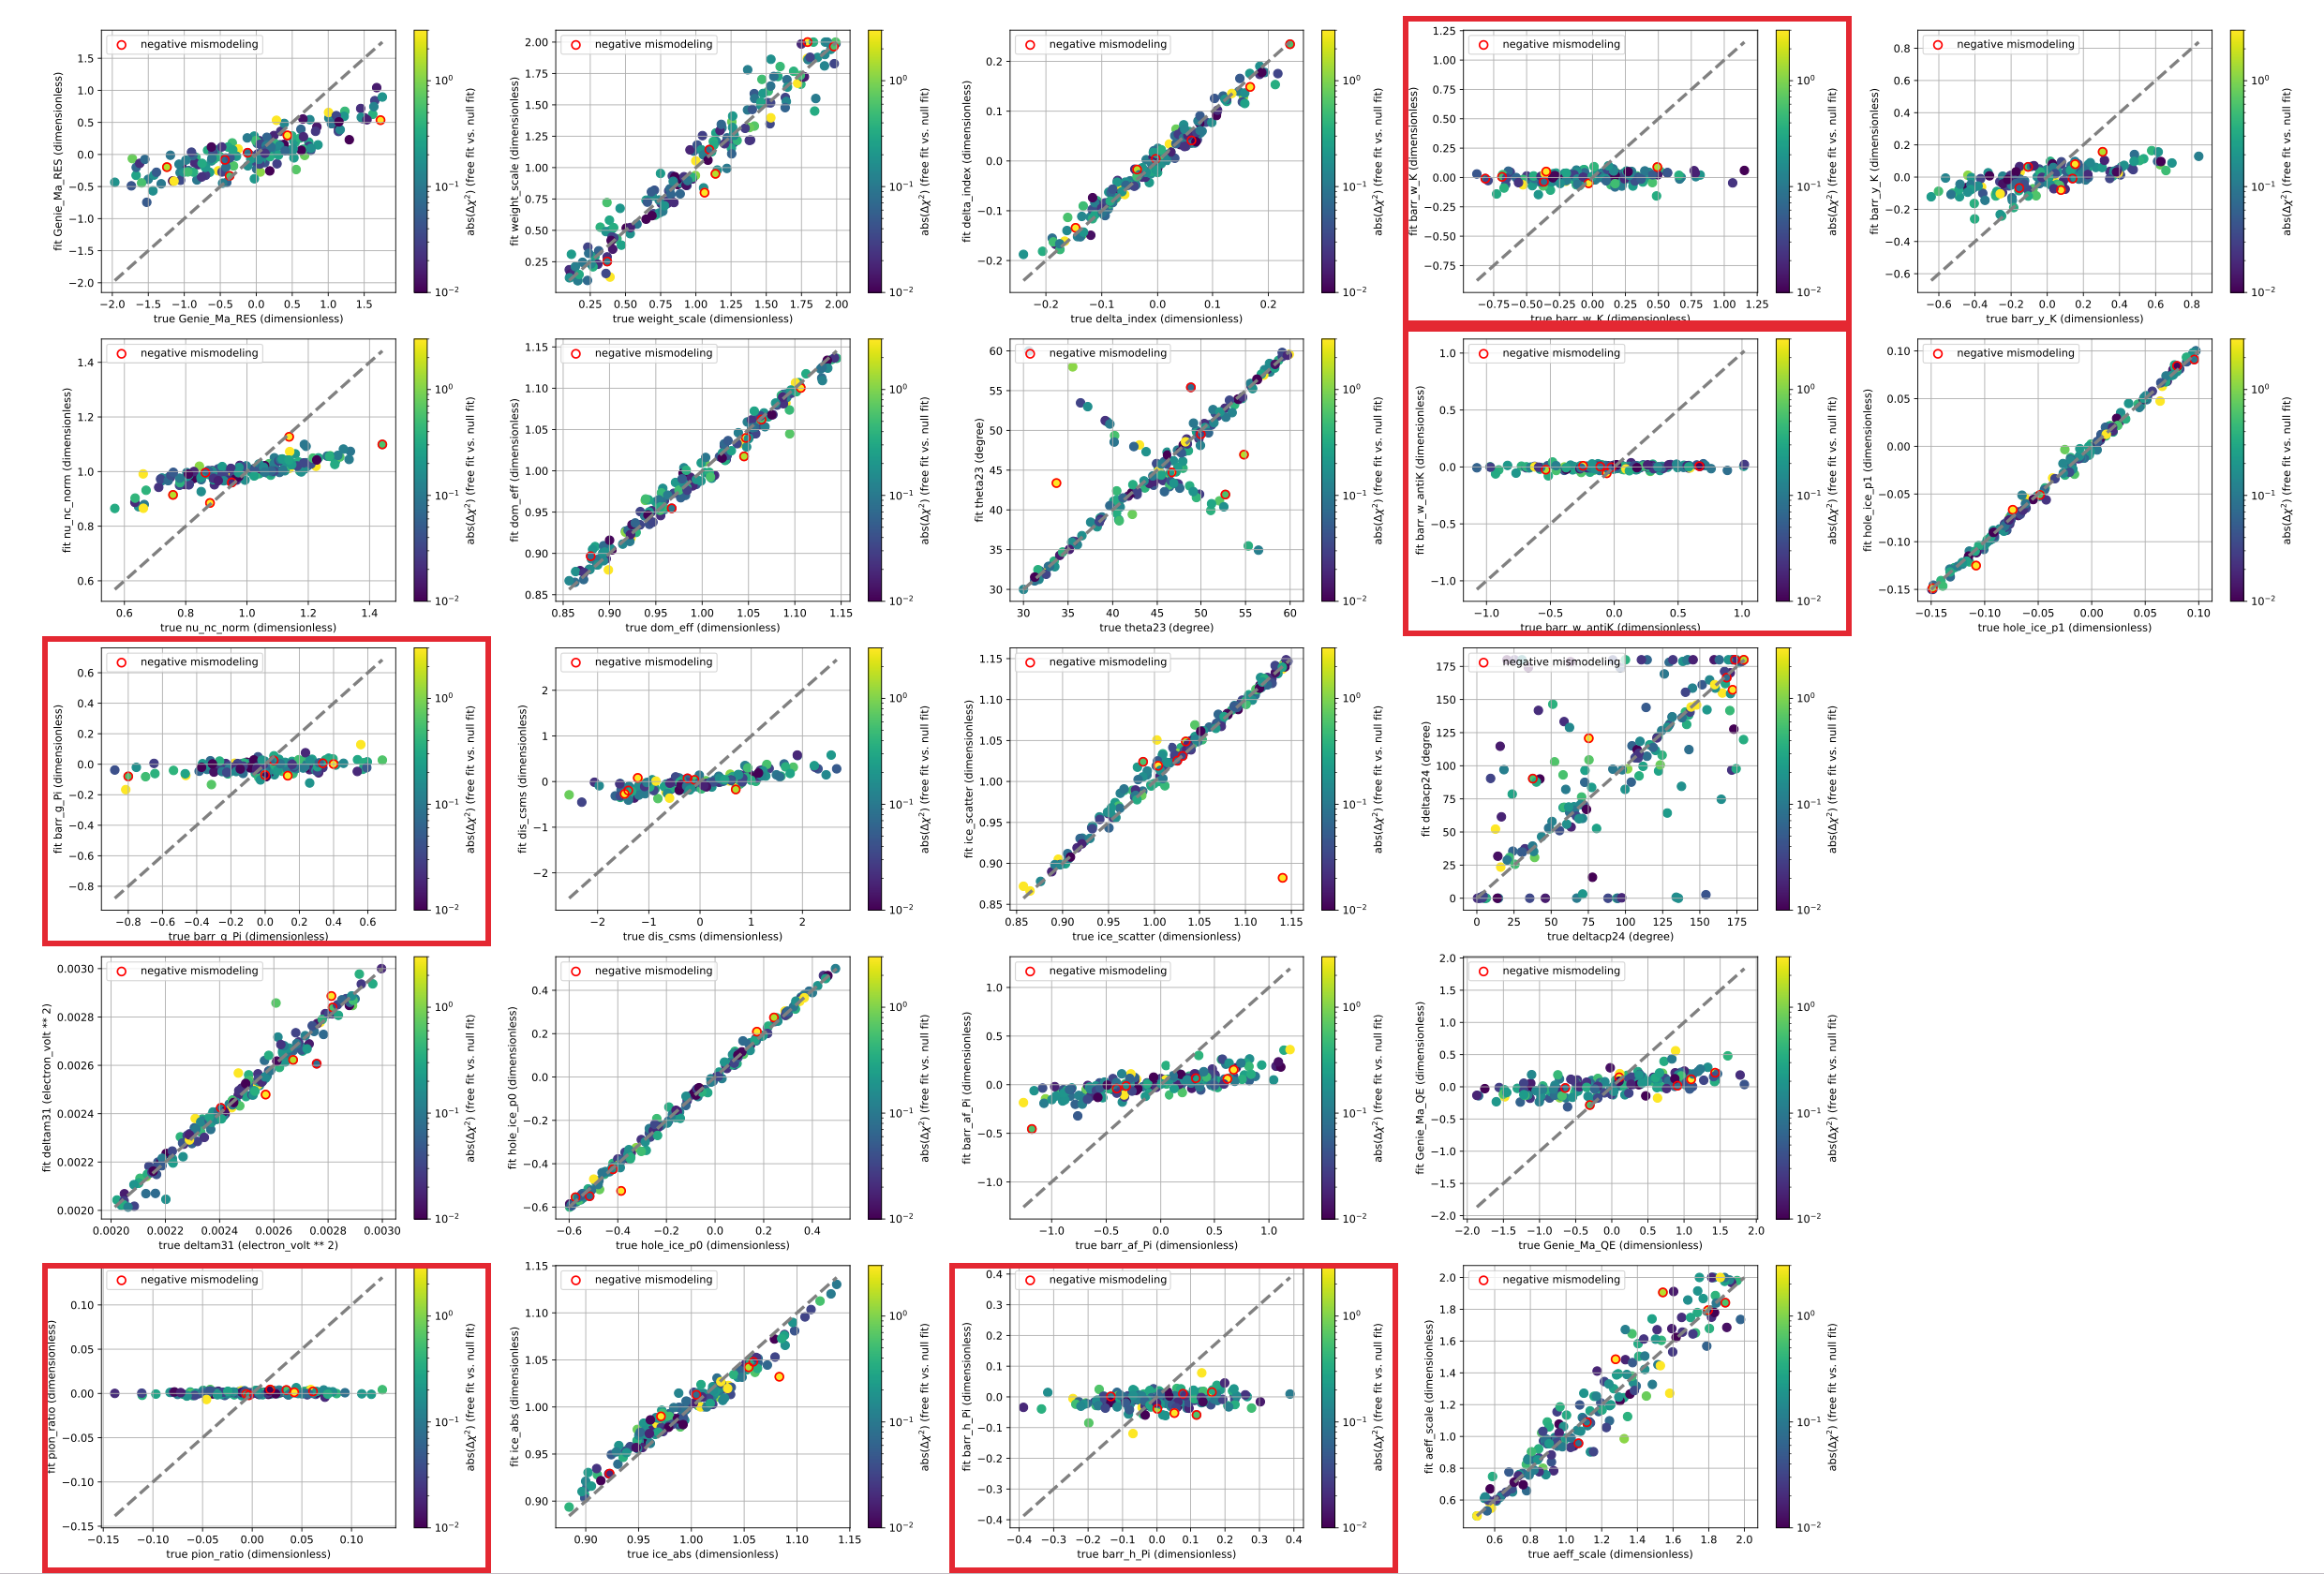
\includegraphics{figures/measurement/sterile_analysis/param_selection/Screen Shot 2022-05-30 at 13.12.49.png}
    \caption{Result of the ensemble test with randomly injected nuisance parameters. This test was run before the priors on \texttt{barr\_i\_Pi}, \texttt{barr\_z\_K}, and \texttt{barr\_z\_antiK} have been inflated as described in section~\ref{section:flux_systs}. Parameters framed in red have been deemed to be negligible for the analysis. The color scale shows the likelihood difference between the free fit and a fit in which the physics parameters ($\theta_{24}$, $\theta_{34}$ have been fixed to their true value. If this number is negative, the trial is circled in red. In such cases, the minimizer failed to find the correct global optimum in the free fit.}
    \label{fig:parameter-ensemble-result}
\end{figure*}

\begin{table}
    \centering
    \begin{tabular}{cccl}\toprule
        \textbf{parameter} & \textbf{nominal value} & \textbf{range} & \textbf{prior} \\
        \midrule
        $\theta_{24}$ &    $0^\circ$ &  $0^\circ$ to $45^\circ$  & uniform \\
        $\theta_{34}$ &    $0^\circ$ &  $0^\circ$ to $45^\circ$  & uniform \\
        $\theta_{23}$ & $49.6^\circ$ & $20^\circ$ to $70^\circ$  & uniform \\
        $\delta_{24}$ &    $0^\circ$ &  $0^\circ$ to $180^\circ$ & uniform \\
        $\Delta m^2_{31}$ & $2.525\times10^{-3}\;\mathrm{eV^2}$ & $(2\,\rm{to}\, 3)\times10^{-3}\;\mathrm{eV^2}$ & uniform \\
        \midrule
        $\Delta \gamma_\nu$ & 0.0 & $-3\sigma$ to $+3\sigma$ &  $\sigma=0.1$  \\
        $\rm{Barr}, \: a-f_{\pi^+}$ & 0.0 & $-3\sigma$ to $+3\sigma$ &  $\sigma=0.63$  \\
        $\rm{Barr}, \: i_{\pi^+}$ & 0.0 & $-3\sigma$ to $+3\sigma$ &  $\sigma=0.61$  \\
        $\rm{Barr}, \: y_{K^+}$ & 0.0 & $-3\sigma$ to $+3\sigma$ &  $\sigma=0.3$  \\
        \midrule
        $M_{A,QE}$ & 0.0 & $-2\sigma$ to $+2\sigma$ &  $\sigma=1.0$  \\
        $M_{A,res}$ & 0.0 & $-2\sigma$ to $+2\sigma$ &  $\sigma=1.0$  \\
        DIS & 0.0 & $-3\sigma$ to $+3\sigma$ &  $\sigma=1.0$  \\
        $N_{\nu, NC}$ & 1.0 & 0.5 to 1.5 &  $\sigma=0.2$  \\
        \midrule
        $N_{\nu}$ & 1.0 & 0.5 to 2.0 & uniform \\
        $N_{\mu}$ & 1.0 & 0 to 3 & uniform \\
        \midrule
        $\epsilon_{\rm{DOM}}$ & 1.0 & 0.85 to 1.15 & $\sigma=0.1$ \\
        $\rm{ice \; absorption}$ & 1.0 & 0.85 to 1.15 & $\sigma=0.05$ \\
        $\rm{ice \; scattering}$ & 1.05 & 0.85 to 1.15 & $\sigma=0.1$ \\
        $\rm{hole \; ice}, \: p_0$ & 0.101569 & -1.1 to 0.5 & uniform \\
        $\rm{hole \; ice}, \: p_1$ & -0.049344 & -0.15 to 0.1 & uniform \\
        \bottomrule
    \end{tabular}
    \caption{List of all free parameters in the sterile oscillation analysis with their respective ranges and priors (if applicable).}
    \label{tab:all-parameters}
\end{table}

\subsubsection{Likelihood Optimization}
The optimization of the likelihood of the sterile oscillation model is considerably more difficult than that of the standard three-flavor oscillation analysis due to the increased complexity of the parameter interactions. Two additional approximate degeneracies arise in the likelihood space from the sterile mixing angles alone: Firstly, for every best fit point in $|U_{\mu 4}|$ and $|U_{\tau 4}|$, there will also be another local optimum where $|U_{\mu 4}|$ and $|U_{\tau 4}|$ are flipped\todo{Add example likelihood scan demonstrating this effect}. In what follows, this is referred to as the \emph{triangle} degeneracy. Secondly, flipping the sign of $\cos(\delta_{24})$, that is, flipping the \emph{quadrant} of $\delta_{24}$ around the angle of $90^\circ$, usually also results in another local minimum. Together with the octant degeneracy of $\theta_{23}$, this means that at least eight local minima have to be checked for every fit. During the development of this analysis, it was found that the likelihood is not entirely convex even within each of these eight distinct segments, leading to a poor performance of local second-order optimizers such as \textsc{migrad}\cite{minuit-algo}. For this reason, the search for the global optimum in this analysis is done in three steps that are run separately for every combination of triangle, quadrant and octant. The first step is a global optimization within each segment of the paraemter space using the CRS2\cite{crs2} algorithm with a population of 300 samples. The optimum found by CRS2 is then taken as the starting point for a local, derivative-free optimization using the \textsc{SbPlx}\cite{subplex} algorithm from the \textsc{nlopt}\cite{nlopt} package. Finally, the best fit point from  \textsc{SbPlx} is used as a starting point to ''polish'' the result using \textsc{migrad}\cite{minuit-algo}. 

\subsection{Analysis Checks}

\subsubsection{Low-pass filtering}
As described in \refsec{low-pass-filtering}, the performance of the oscillation calculation is greatly improved by applying low-pass filters when evaluating the vacuum part of the Hamiltonian. To ensure that the chosen cut-off points of these filters do not introduce significant distortions to the oscillation signal, an inject/recover test is performed on a grid in $|U_{\mu 4}|$ and $|U_{\tau 4}|$ where pseudo-data is produced \emph{without} any low-pass filtering and fit back with the filtering enabled. For every grid point, a second fit is run where $\theta_{24}$ and $\theta_{34}$ are fixed to their true injected values. The p-value of the difference in the test statistic between these two fits, $\Delta \chi^2_{\mathrm{mod}}$, can be interpreted as the significance with which the true value of the mixing angles would be rejected solely due to the mis-modeling of the true oscillation probabilities. The fit results of the mixing parameters and the corresponding values of $\Delta \chi^2_{\mathrm{mod}}$ are shown in \reffig{asimov-test-sterile-ana}. Assuming that $\Delta \chi^2_{\mathrm{mod}}$ should follow a $\chi^2$ distribution with two degrees of freedom, the significance of the mis-modeling is very small. The visible fit errors for small values of $|U_{\mu 4}|$ and $|U_{\tau 4}|$ are insignificant because the likelihood is very flat in this region of the parameter space.

\begin{figure*}
    \centering
    \missingfigure[figwidth=0.9\linewidth, figheight=0.4\linewidth]{Inject/recover results and mis-modeling plot for sterile analysis}
    \caption{Results of the inject/recover test (left) and the corresponding mis-modeling values, $\Delta \chi^2_{\mathrm{mod}}$, attributable to low-pass filtering in \textsc{nuSQuIDS} (right).}
    \label{fig:asimov-test-sterile-ana}
\end{figure*}

\subsubsection{Fit Convergence}

The inject/recover test with randomly sampled physics and nuisance parameters that is described in \refsec{sterile-analysis-parameter-selection} is used to quantify the reliability with which the correct global optimum is be found. To do this, a second fit is run for each trial where the values of $\theta_{24}$ and $\theta_{34}$ are fixed to their true values. If the test statistic for this fit is smaller than that of the free fit, then the global optimization is proven to have failed to find the correct optimum. Trials for which this is the case are marked in \reffig{parameter-ensemble-result} with red circles as having negative mis-modeling values. It is apparent from \reffig{parameter-ensemble-result} that this is the case for a small percentage of trials. The failure rate decreases after the parameters framed in red are fixed. With the final parameter selection and minimization scheme, the rate of minimization failure found in this test is X\%\todo{Find fraction of failed fits for final selection}. Because it is not possible to generally prove the success of a fit, the failure rate of this test can only provide a lower bound to the true failure rate. The failure rate of the optimization could be reduced by either splitting the likelihood space into even more chunks, or by increasing the number of samples used by the \textsc{CRS2} search, but only at a significant increase to the already considerable computational cost of the analysis. 

\subsection{Results}

Just as the three-flavor oscillation analysis, the results of the sterile oscillation analysis are revealed in a staged procedure. The best fit values of the sterile mixing parameters are only revealed after convergence of the minimizer and a good fit quality has been verified.

\subsubsection{Minimizer Convergence}
The first stage is to ensure that the likelihood optimization has properly converged by running a second fit where the physics parameters are fixed to the best fit point of the free fit. The best fit parameter values and the test statistic of both fits are compared with a script that only prints the differences between them without revealing their absolute values to the analyzer. As expected, this fit converges to the same parameter values and test statistic value as the free fit to within the tolerance of the minimizer.

\subsubsection{Goodness of Fit}
In a similar fashion as for the three-flavor oscillation analysis, the goodness-of-fit is established using an ensemble of pseudo-data trials with fluctuations taking both the MC uncertainty and the Poisson fluctuation of the data into account. The pseudo-data expectation is generated by injecting the best fit values of the real data fit as true values. The distribution of test statistic values resulting from this ensemble compared to that of the real data fit is shown in \reffig{sterile-modchi2-ensemble-comparison}. The p-value of the observed test statistic is 22.5\%, demonstrating that the goodness of fit is well within the expectation. 

\begin{figure}
    \centering
    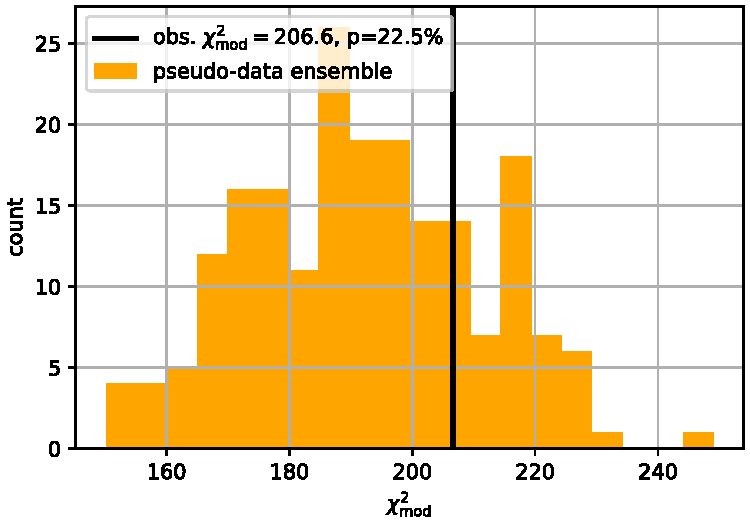
\includegraphics[width=0.8\linewidth]{figures/measurement/sterile_analysis/results/compare_ts_to_ensemble_REAL_DATA_FIT_v12_ext_holeice.pdf}
    \caption{Observed test statistic compared to the distribution expected from pseudo-data trials for the sterile oscillation analysis.}
    \label{fig:sterile-modchi2-ensemble-comparison}
\end{figure}

\subsubsection{Likelihood Scan and Contour}
The likelihood is scanned over $|U_{\mu 4}|$ and $|U_{\tau 4}|$ while marginalizing over all other parameters, including the standard three-flavor oscillation parameters and $\delta_{24}$. The degeneracies in $\theta_{23}$ and $\delta_{24}$ are broken by running four separate fits, one for each possible combination of octant and quadrant. One additional local \textsc{migrad} optimization is run for every grid point of the scan in which all nuisance parameters start from the global best fit point. The test statistic value used in the scan is the optimum out of these five fits. Contours are drawn assuming Wilks' theorem with two degrees of freedom. This assumption is certainly violated in some parts of the parameter space, especially in regions of very small sterile mixing due to boundary effects and the fact that the CP-violating phase $\delta_{24}$ can no longer provide a degree of freedom if either mixing amplitude is zero. However, since the contour line to be drawn lies mostly in regions where neither $\theta_{24}$ nor $\theta_{34}$ are close to zero, Wilks' theorem still provides a useful approximation. The coverage of the assumed $\chi^2$ distribution is tested on three points along the contour to determine if it is over-covering or under-covering. The test statistic value at every scan point and the resulting contours for the 90\% and 99\% C.L. are shown in \reffig{sterile-contour-scan}. For both $|U_{\mu 4}|$ and $|U_{\tau 4}|$, the analysis can constrain the amplitude of active-sterile mixing to $<0.1$ at $>99\%$ C.L., setting the strongest limit on $|U_{\tau 4}|$ to date. 

\begin{figure}
    \centering
    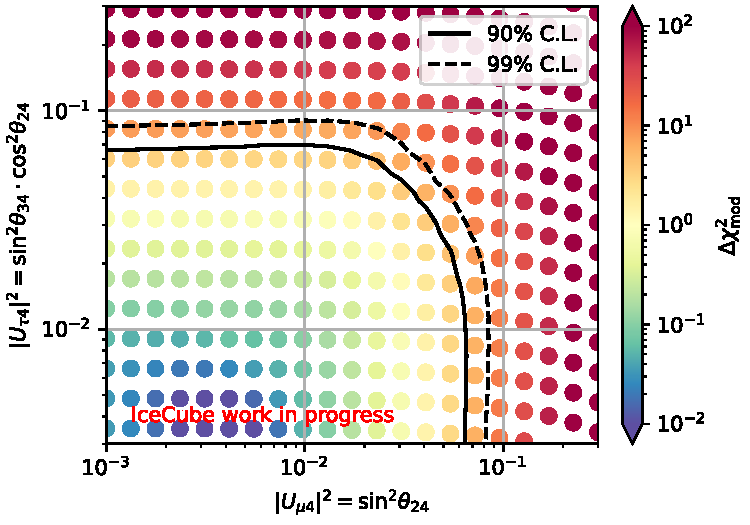
\includegraphics{figures/measurement/sterile_analysis/results/REAL_DATA_wilks_contours_merged_scans.pdf}
    \caption{Scan of the $\chi^2_{\mathrm{mod}}$ difference with respect to the best fit point with 90\% and 99\% C.L. contours assuming Wilks' theorem with two degrees of freedom.}
    \label{fig:sterile-contour-scan}
\end{figure}